\documentclass[final,oneside,onecolumn]{article}
\usepackage[body={6in,9.5in},top=0.9in,left=1in,dvips]{geometry}
\usepackage{amsmath}
\usepackage{amsthm}
\usepackage{mathtools}
\usepackage{float}
\usepackage{graphicx}
\usepackage{amsfonts}
\usepackage{amssymb}
\usepackage{paralist}
\usepackage{floatflt}
\usepackage{alltt}

\usepackage{caption}
\usepackage{subcaption}

\usepackage{algorithmic}
\usepackage{blkarray}

%\usepackage{algorithm}
%\usepackage{algorithmic}
\usepackage{url}
\usepackage{xspace}

% lstlisting
\usepackage{listings}
\usepackage{upquote} % Fixes single quotes in Verbatum environments
\usepackage{courier}
\usepackage{color}
\definecolor{string}{rgb}{0.7,0.0,0.0}
\definecolor{comment}{rgb}{0.13,0.54,0.13}
\definecolor{keyword}{rgb}{0.0,0.0,1.0}

% Python LstListing
\definecolor{pygreen}{rgb}{0,.4,0}
\definecolor{pyoperator}{rgb}{.8,0,.8}
\definecolor{pycomment}{rgb}{.5,.5,.5}
\definecolor{pyidentifier}{rgb}{0,0,1}
\lstset{language=Python,
	showstringspaces=false,
	numbers=left,
	breaklines=true,
	tabsize=4,
    keywordstyle=\color{pygreen},
    stringstyle=\color{string},
    commentstyle=\color{pycomment},
    %identifierstyle=\color{pyidentifier},
    literate=    {+}{{{\color{pyoperator}+}}}{1}
    {*}{{{\color{pyoperator}*}}}{1}
    {-}{{{\color{pyoperator}-}}}{1}
    {/}{{{\color{pyoperator}/}}}{1}
    {**}{{{\color{pyoperator}**}}}{2}
    {@}{{{\color{pyoperator}@}}}{1},
    basicstyle=\footnotesize\ttfamily\bfseries
}
% Fortran LstListing
\lstset{language=[90]Fortran,
	basicstyle=\ttfamily\bfseries,
	keywordstyle=\color{blue},
	commentstyle=\color{pygreen},
	morecomment=[l]{!\ }% Comment only with space after !
}


\newcommand{\matlab}{{\sc Matlab}\xspace}
\newcommand{\matlabs}{\textsc{Matlab}'s\xspace}
\newcommand{\grads}{[\text{565 only}]}
\newcommand{\ugrads}{[\text{465 only}]}
\newcommand{\maple}{\emph{Maple\;}}
\newcommand{\erf}{\text{erf}}
\newcommand{\sign}{\text{sign}}
\newcommand{\lnorm}{\left\|}
\newcommand{\rnorm}{\right\|}
\newcommand{\ds}{\displaystyle}
\newcommand{\lam}{\lambda}
\newcommand{\ol}{\overline}
\newcommand{\vf}{\mathbf{f}}
\newcommand{\vy}{\mathbf{y}}
\newcommand{\vx}{\mathbf{x}}
\newcommand{\vd}{\mathbf{d}}
\newcommand{\sn}{\text{sn}}
\newcommand{\cn}{\text{cn}}
\newcommand{\dn}{\text{dn}}

\newcommand{\fdst}[3]{\left[\begin{array}{ccc} #1 & #2 & #3 \end{array}\right]}

%%%%%%%%%%%%%%%%%%%%%%%%%%%%%%%%%%%%%%%%%%%%%%%%%%%%%%%%%%%%%%%%%%%%%%%%%%%%%%%%%%%%%%%%%%%%%%%%%%%%
% Commands and Custom Variables	
\newcommand{\problem}[1]{{\parindent=-2em \large \textbf{Problem #1} }}
%\newcommand{\problemnocollab}[1]{\hspace{-4 ex} \large \textbf{Problem #1: No Collaboration} }
\newcommand{\problemnocollab}[1]{{\parindent=-2em \large \textbf{Problem #1: No Collaboration} }}
\newcommand{\problemcollab}[2]{{\parindent=-2em \large \textbf{Problem #1: Collaboration Allowed}} \\ {\large \textbf{Collaborators:} #2\bigbreak} }
\let\oldemptyset\emptyset
\let\emptyset\varnothing
\newcommand{\norm}[1]{\left\lVert#1\right\rVert}
\newcommand{\sint}{\text{s}\kern-5pt\int}
\newcommand{\powerset}{\mathcal{P}}
\renewenvironment{proof}{\hspace{-4 ex} \emph{Proof}:}{\qed}
\newcommand{\FF}{\mathcal{F}}
\newcommand{\RR}{\mathbb{R}}
\newcommand{\NN}{\mathbb{N}}
\newcommand{\OO}{\mathcal{O}}
\newcommand{\mathcow}{\OO}
\newcommand{\QQ}{\mathbb{Q}}
\newcommand{\ZZ}{\mathbb{Z}}
\newcommand{\CC}{\mathbb{C}}
\newcommand{\KK}{\mathbb{K}}
\newcommand{\PP}{\mathcal{P}}
\newcommand{\TT}{\mathcal{T}}
\newcommand{\BB}{\mathcal{B}}
\newcommand{\LL}{\mathcal{L}}
\renewcommand{\Re}{\operatorname{Re}}
\renewcommand{\Im}{\operatorname{Im}}

\newcommand{\veca}{\vec{a}}
\newcommand{\vecb}{\vec{b}}
\newcommand{\vecd}{\vec{d}}
\newcommand{\vece}{\vec{e}}
\newcommand{\vecf}{\vec{f}}
\newcommand{\vecn}{\vec{n}}
\newcommand{\vecp}{\vec{p}}
\newcommand{\vecr}{\vec{r}}
\newcommand{\vecu}{\vec{u}}
\newcommand{\vecv}{\vec{v}}
\newcommand{\vecx}{\vec{x}}
\newcommand{\vecy}{\vec{y}}
\newcommand{\vecz}{\vec{z}}

\newcommand{\range}{\text{range}}
\newcommand{\kernel}{\text{ker}}
\newcommand{\vspan}{\text{span}}

\newcommand{\solution}{\vspace{2 ex} \hspace{-9 ex} \emph{Solution.} }

\newcommand{\sech}{\text{ sech}}

\DeclareMathOperator*{\argmax}{arg\,max}
\DeclareMathOperator*{\argmin}{arg\,min}

\renewcommand{\vec}[1]{\mathbf{#1}}

\newcommand{\hr}{\makebox[\linewidth]{\rule{.8\paperwidth}{0.4pt}}}

\newcommand{\comment}[1]{\textcolor{red}{\textbf{\MakeUppercase{#1}}}}

\newtheorem{lemma}{Lemma}

\graphicspath{{images/}}

% dashint
\def\Xint#1{\mathchoice
	{\XXint\displaystyle\textstyle{#1}}%
	{\XXint\textstyle\scriptstyle{#1}}%
	{\XXint\scriptstyle\scriptscriptstyle{#1}}%
	{\XXint\scriptscriptstyle\scriptscriptstyle{#1}}%
	\!\int}
\def\XXint#1#2#3{{\setbox0=\hbox{$#1{#2#3}{\int}$ }
		\vcenter{\hbox{$#2#3$ }}\kern-.6\wd0}}
\def\ddashint{\Xint=}
\def\dashint{\Xint-}

\begin{document}

\renewcommand{\arraystretch}{1}

\title{\begin{tabular*}{6.5in}[h]{l@{\extracolsep\fill}cr}
{\bf \large Python Code Samples} & {\bf \large \LaTeX \ Integration} &  {\bf \large Sage Shaw}\\
& {\bf \large \today} \\
\end{tabular*}}
\date{}
\author{}
\maketitle

%\begin{figure}[!b]
%	\centering
%	\includegraphics[width=1.0\textwidth]{HW01_problem2a.eps}
%	\caption{Order $\OO(\varepsilon)$ approximations (three terms) to the roots of $\varepsilon^3x^2 + \varepsilon x + 1 = 0$ from problem 2a.}
%	\label{fig:2a}
%\end{figure}

\thispagestyle{empty}
\bigbreak
%%%%%%%%%%%%%%%%%%%%%%%%%%%%%%%%%%%%%%%%%%%%%%%%%%%%%%%%%%%%%%%%%%

This document demonstrates the techniques discussed in the Python Code Samples for integrating python code and code output into \LaTeX documents.

%%%%%%%%%%%%%%%%%%%%%%%%%%%%%%%%%%%%%%%%%%%%%%%%%%%%%%%%%%%%%%%%%%
\section{Images}

Figure \ref{fig:formats} demonstrates the use of the .eps and .png file formats. The files were generated using the same MatPlotLib code, which created a small figure. The .eps file renders a high-resolution file, whereas the .png image appears blurry when scaled. Use the .eps file format when inserting figures into \LaTeX documents. 

{\bf Note:} Encapsulated Post Script has inerrant vulnerabilities. Do not compile .eps files obtained from untrusted sources.

\begin{figure}
	\begin{subfigure}[b]{\textwidth}
		\centering
		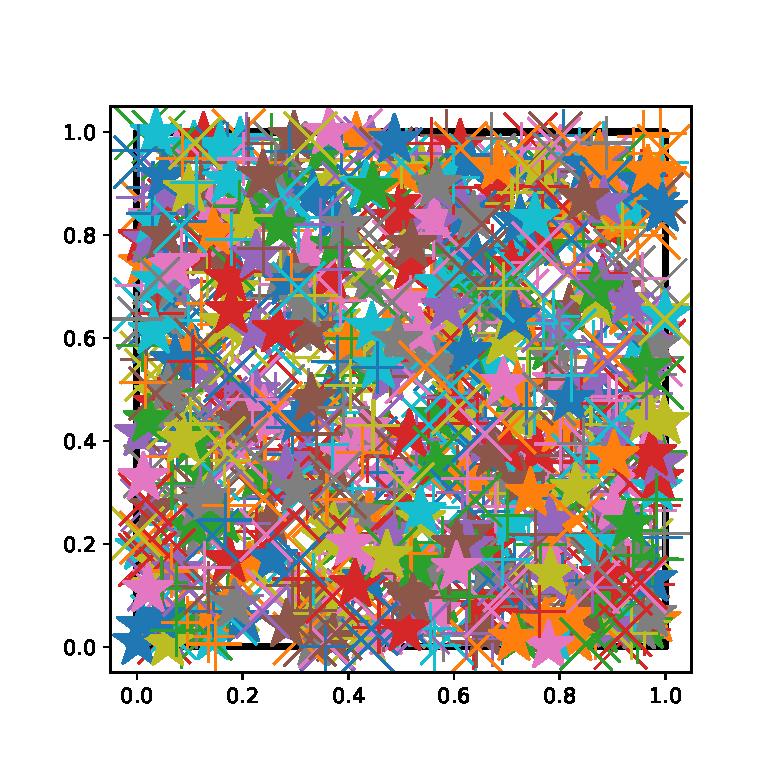
\includegraphics[width=0.7\textwidth]{test.eps}
		\caption{Encapsulated Post Script}
		\label{fig:eps}
	\end{subfigure}
	\hfill
	\begin{subfigure}[b]{\textwidth}
			\centering
			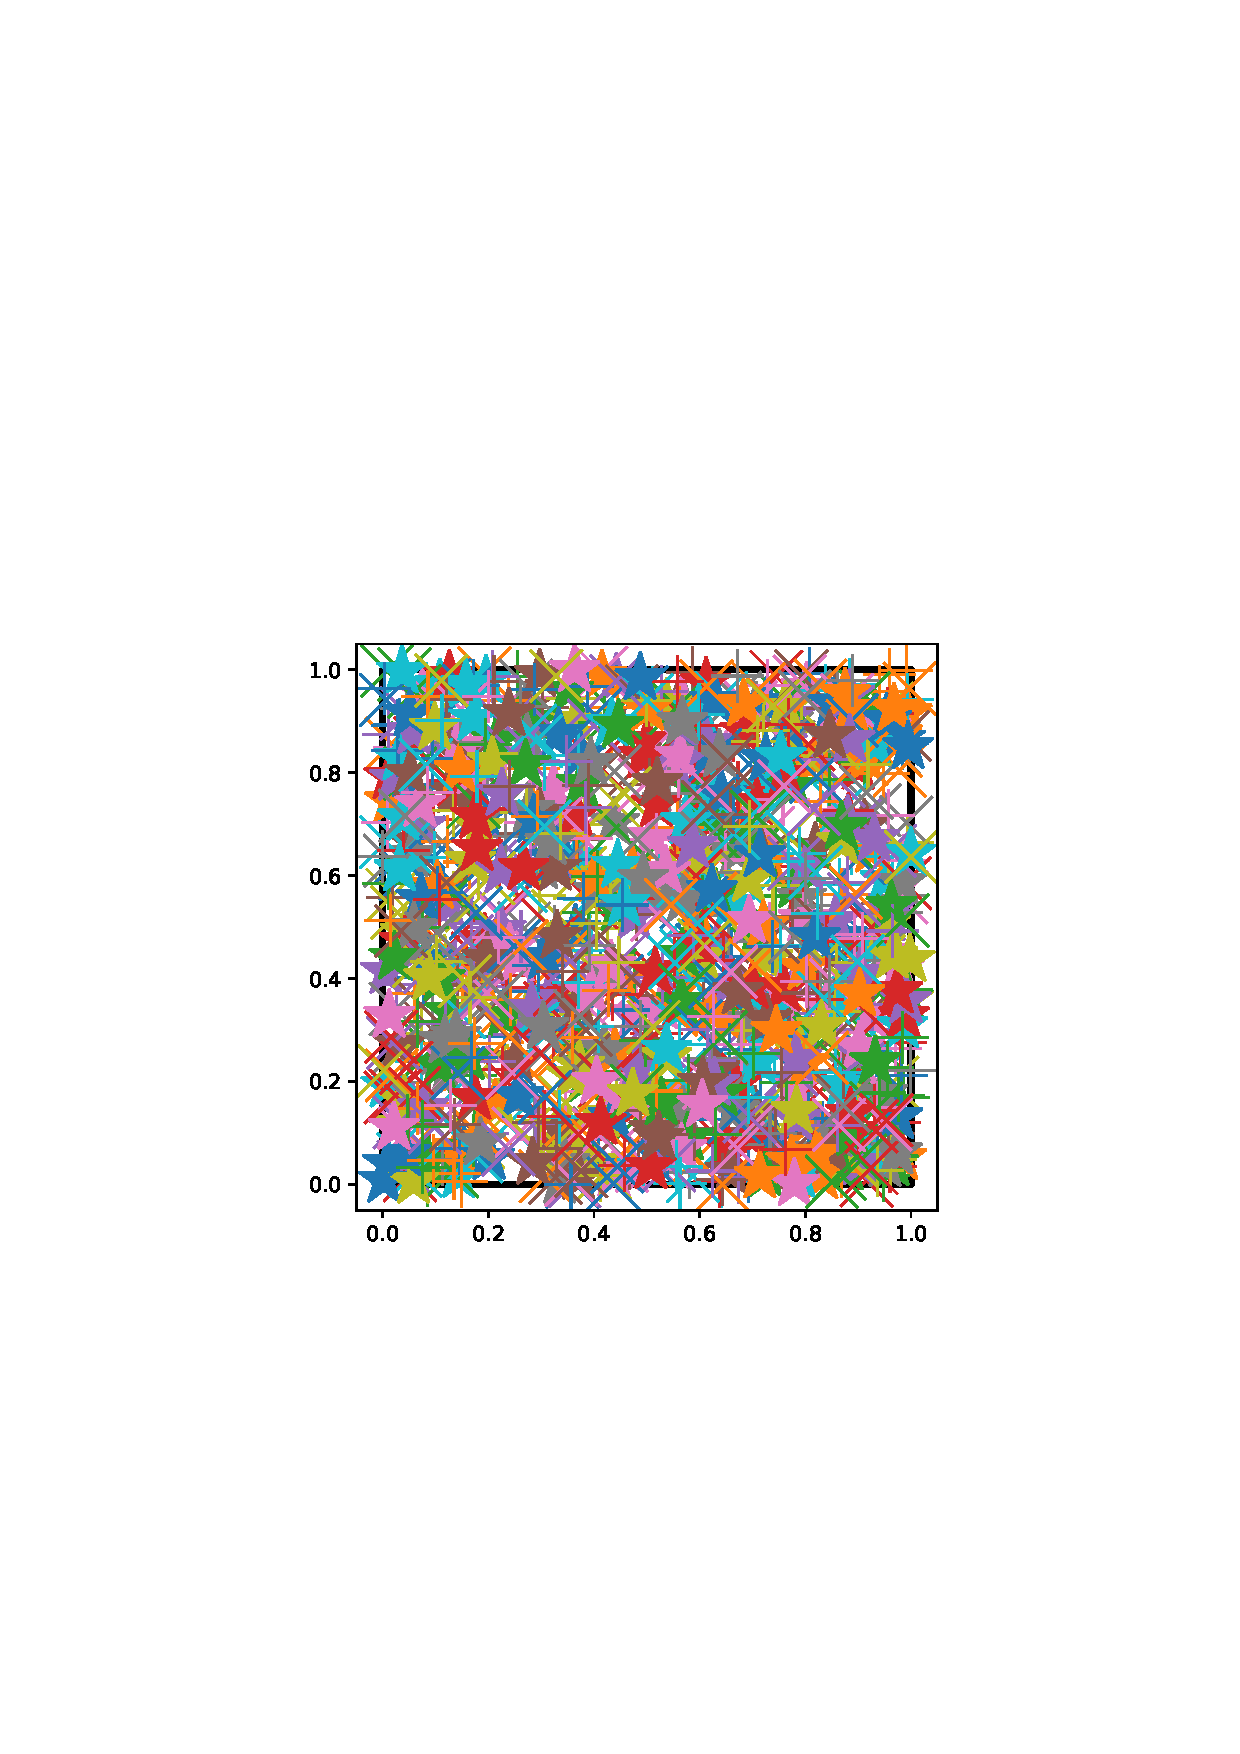
\includegraphics[width=.7\textwidth]{test.png}
			\caption{PNG}
			\label{fig:png}
		\end{subfigure}
	\caption{Resolution differences between .eps and .png files.}
	\label{fig:formats}
\end{figure}

\end{document}